
\documentclass[letterpaper, reqno,11pt]{article}
\usepackage[margin=1.0in]{geometry}
\usepackage{color,latexsym,amsmath,amssymb}
\usepackage{fancyhdr}
\usepackage{amsthm}
\usepackage{mathtools}
\usepackage{tikz}
\usepackage{float}
\usepackage{centernot}
\usepackage{subcaption}
\usepackage{extarrows}
\usetikzlibrary{hobby}
\usetikzlibrary{shapes.multipart}
\usepackage{pgfplots}
\pgfplotsset{compat=1.7}
\usetikzlibrary{arrows.meta}
\usepackage{cancel}
\usetikzlibrary{decorations.markings}
\usetikzlibrary{shapes}
\usetikzlibrary{arrows}
\usepgfplotslibrary{fillbetween}
\usetikzlibrary{patterns}

\newcommand{\RR}{\mathbb{R}}
\newcommand{\CC}{\mathbb{C}}
\newcommand{\ZZ}{\mathbb{Z}}
\newcommand{\QQ}{\mathbb{Q}}
\newcommand{\NN}{\mathbb{N}}
\DeclareMathOperator{\id}{id}
\def\upint{\mathchoice%
  {\mkern13mu\overline{\vphantom{\intop}\mkern7mu}\mkern-20mu}%
  {\mkern7mu\overline{\vphantom{\intop}\mkern7mu}\mkern-14mu}%
  {\mkern7mu\overline{\vphantom{\intop}\mkern7mu}\mkern-14mu}%
  {\mkern7mu\overline{\vphantom{\intop}\mkern7mu}\mkern-14mu}%
  \int}
\def\lowint{\mkern3mu\underline{\vphantom{\intop}\mkern7mu}\mkern-10mu\int}
\DeclareMathOperator{\card}{card}
\DeclareMathOperator{\Binomial}{Binomial}
\DeclareMathOperator{\Span}{span}
\DeclareMathOperator{\sgn}{sgn}
\pagestyle{fancy}
\lhead{Math 321 Lecture 30}
\rhead{Yuchong Pan}
\begin{document}
\pagenumbering{arabic}
\title{Math 321 Lecture 30}
\author{Yuchong Pan}
\date{March 22, 2019}
\newtheorem{thm}{Theorem}
\newtheorem{defn}{Definition}
\newtheorem*{remark}{Remark}
\newtheorem{claim}{Claim}
\newtheorem{cor}{Corollary}
\newtheorem{lemma}{Lemma}
\newtheorem{prop}{Proposition}
\newtheorem{fact}{Fact}
\maketitle
%

\section{Proof of the Inverse Function Theorem (Cont'd)}

\begin{proof}[Proof (Cont'd)]
  \renewcommand{\qedsymbol}{}
  
  Let
  \[ \mathbf f : E \to \RR^n, \qquad E \overset{\text{open}}{\subseteq} \RR^n, \qquad \mathbf a \in E, \qquad \mathbf A = \mathbf f'(\mathbf a) \text{ invertible}, \qquad \underbrace{\mathbf f \in C^1(E)}_{\substack{\text{$\Leftrightarrow$ $x \mapsto \mathbf f'(x)$ is continuous on $E$:} \\ \text{given any $\lambda > 0$, there exists $\delta > 0$} \\ \text{such that $\lVert \mathbf f'(\mathbf x) - \mathbf A \rVert < \lambda$ for $\lVert \mathbf x - \mathbf a \rVert < \delta$}}}. \]

  \begin{enumerate}
  \item Last time, we found $U = B(\mathbf a, \epsilon)$ and $V = \mathbf f(U)$ such that $\mathbf f : U \to V$ is a bijection. We showed $\mathbf f$ is $1$-$1$ on $U$ using the CMP. Defined $\varphi_{\mathbf y}(\mathbf x) = \mathbf x + \mathbf A^{-1} (\mathbf y - \mathbf f(\mathbf x)), \mathbf x \in E$; showed that for $\mathbf x_1, \mathbf x_2 \in U$,
    \begin{equation} \label{eq:*} \tag{*}
      \boxed{\lVert \varphi_{\mathbf y} (\mathbf x_1) - \varphi_{\mathbf y}(\mathbf x_2) \rVert \leq \frac{1}{2} \lVert \mathbf x_1 - \mathbf x_2 \rVert.}
    \end{equation}
    Note that
    \[ \lVert \varphi_{\mathbf y}(\mathbf x_1) - \varphi_{\mathbf y}(\mathbf x_2) \rVert \leq \lVert \varphi_{\mathbf y}' \rVert \cdot \lVert \mathbf x_1 - \mathbf x_2 \rVert, \]
    where
    \[ \lVert \varphi_{\mathbf y}'(\mathbf x) \rVert = \lVert \mathbf I - \mathbf A^{-1} \mathbf f'(\mathbf x) \rVert = \left\lVert \mathbf A^{-1} (\mathbf A - \mathbf f'(\mathbf x)) \right\rVert. \]
    Pick $\epsilon > 0$ so that
    \[ \underbrace{\lVert \mathbf x - \mathbf a \rVert < \epsilon}_{\mathbf x \in U} \Rightarrow \lVert \mathbf A - \mathbf f'(\mathbf x) \rVert < \frac{1}{2 \lVert \mathbf A^{-1} \rVert}. \]
    Thus,
    \[ \lVert \varphi_{\mathbf y}'(\mathbf x) \rVert \leq \left\lVert \mathbf A^{-1} \right\rVert \cdot \lVert \mathbf A - \mathbf f'(\mathbf x) \rVert < \left\lVert \mathbf A^{-1} \right\rVert \cdot \lambda = \frac{1}{2}. \]

    \noindent {\bf Remark:} The $\epsilon$ chosen to define $U = B(\mathbf a, \epsilon)$ is independent of $\mathbf y$, but dependent on $\mathbf a$ and $\mathbf f$.

    \noindent \fbox{\begin{minipage}{\textwidth}
        \noindent {\bf Remark:} Let $V, W$ be vector spaces.
        \[ \text{$\mathbf B : V \xrightarrow{\text{linear}} W$ where $\dim(V) < \infty, \dim(W) < \infty$} \Rightarrow \text{$\mathbf B$ is continuous and bounded; i.e., $\lVert \mathbf B \rVert < \infty$.} \]
      \end{minipage}
    }

    \eqref{eq:*} is a contraction condition, but $\varphi_{\mathbf y}$ need not map $U$ to itself.

    \noindent {\bf Note:} $U$ is not complete, but $\overline U$ is. \eqref{eq:*} continues to hold for $\mathbf x_1, \mathbf x_2 \in \overline U$.

    \noindent Can $\varphi_{\mathbf y}$ have a fixed point in $U$?

    \noindent If there exists such $\mathbf x$, then
    \[ \varphi_{\mathbf y}(\mathbf x) = \mathbf x \in U \Rightarrow \varphi_{\mathbf y}(\mathbf x) \in U. \]
    We do not know if $\varphi_{\mathbf y}(U) \subseteq U$, so cannot guarantee the \emph{existence} of a fixed point of $\varphi_{\mathbf y}$. However, \fbox{if a fixed point exists}, by CMP it would have to be unique.

    Take $\mathbf y \in V = \mathbf f(U)$. Then there exists $\mathbf x \in U$ such that $\mathbf f(\mathbf x) = \mathbf y$. Thus, $\mathbf x$ is a fixed point of $\varphi_{\mathbf y}$. By CMP, there exists only one such $\mathbf x$; hence $\mathbf f: U \to V$ is injective.

    \begin{figure}[H]
      \centering
      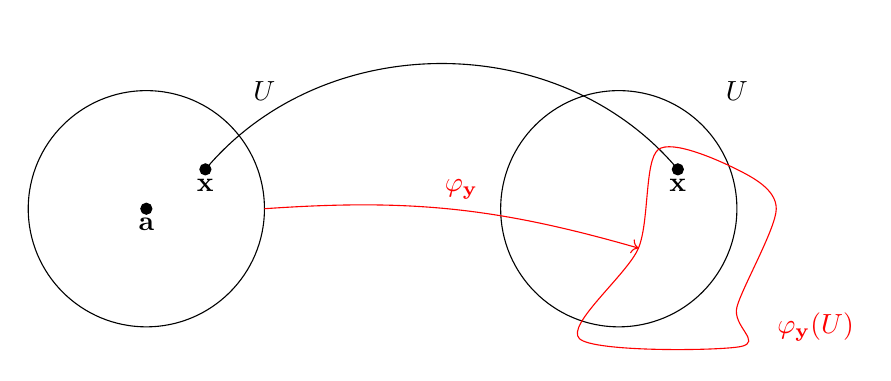
\begin{tikzpicture}
        \draw (0, 0) circle (1.5);
        \draw (6, 0) circle (1.5);
        \draw[fill=black] (0, 0) circle (2pt) node[below] {$\mathbf a$};
        \draw[fill=black] (0.75, 0.5) circle (2pt) node[below] {$\mathbf x$};
        \draw[fill=black] (6.75, 0.5) circle (2pt) node[below] {$\mathbf x$};
        \node at (1.5, 1.5) {$U$};
        \node at (7.5, 1.5) {$U$};
        \draw (0.75, 0.5) to[bend left=50] (6.75, 0.5);
        \draw[red] plot [mark=none, smooth cycle] coordinates {(6.5, 0.75) (7.5, 0.5) (8, 0) (7.5, -1.25) (7.55, -1.75) (5.5, -1.65) (6.25, -0.5)};
        \node[red] at (8.5, -1.5) {$\varphi_{\mathbf y}(U)$};
        \draw[->, red] (1.5, 0) to[bend left=10] (6.25, -0.5);
        \node[red] at (4, 0.25) {$\varphi_{\mathbf y}$};
      \end{tikzpicture}
    \end{figure}

    \noindent {\bf Exercise:} $V$ is open.

  \item Let $\mathbf g : V \to U$ where $\mathbf g = \mathbf f^{-1}$ defined by part (a). Want to show $\mathbf g$ is differentiable on $V$; in fact, $\mathbf g \in C^1(V)$.

    \noindent \emph{Proof.} Need to find $\mathbf T = \mathbf T(\mathbf y)$ continuous on $V$ such that
    \[ \frac{\lVert \mathbf g(\mathbf y + \mathbf k) - \mathbf g(\mathbf y) - \mathbf T \mathbf k \rVert}{\lVert \mathbf k \rVert} \xrightarrow{\lVert \mathbf k \rVert \to 0} 0. \]

    \fbox{\begin{minipage}{\textwidth}
        In $\RR$,
        \[ g \circ f(x) = x \Rightarrow g'(f(x)) \cdot f'(x) = 1 \Rightarrow g'\left(\underbrace{f(x)}_y\right) = \frac{1}{\underbrace{f'(x)}_{f'(f^{-1}(y))}}. \]
      \end{minipage}
    }

    Choose $\mathbf T = (\mathbf f'(\mathbf g(\mathbf y)))^{-1}$. We will show that $\mathbf T$ is well-defined.

    \noindent {\bf Recall:} A matrix $\mathbf B_{n \times n}$ is invertible if and only if $\underbrace{\det(\mathbf B)}_{\substack{\text{a polynomial in the entries of $\mathbf B$} \\ \text{hence continuous in the entries of $\mathbf B$}}} \neq 0$.

    Hence, $\mathbf x \in E \subseteq \RR^n \mapsto \det(\mathbf f'(\mathbf x)) \in \RR$ is a continuous map, which assumes a nonzero value at $\mathbf x = \mathbf a$. Hence it remains nonzero on $U = B(\mathbf a, \epsilon)$ for $\epsilon > 0$ small.

    Set
    \begin{align*}
      \mathbf f(\mathbf x) = \mathbf y \in V & \Leftrightarrow \mathbf g(\mathbf y) = \mathbf x, \\
      \mathbf f(\mathbf x + \mathbf h) = \mathbf y + \mathbf k & \Leftrightarrow \mathbf g(\mathbf y + \mathbf k) = \mathbf x + \mathbf k.
    \end{align*}
    Then,
    \[ \mathbf g(\mathbf y + \mathbf k) - \mathbf g(\mathbf y) - \mathbf T \mathbf k = \mathbf h - \mathbf T \mathbf k = \mathbf T \left(\mathbf T^{-1} \mathbf h - \mathbf k\right) = \mathbf T(\mathbf f'(\mathbf x) \mathbf h - \mathbf k) = \mathbf T\left(\underbrace{(\mathbf f(\mathbf x) - \mathbf f'(\mathbf a)) \mathbf h}_\text{I} + \underbrace{\mathbf f'(\mathbf a) \mathbf h - \mathbf k}_\text{II}\right). \]
    
    Want to show that
    \begin{equation} \label{eq:??}
      \frac{\lVert \text{II} \rVert}{\lVert \mathbf k \rVert} = \frac{\mathbf T(\mathbf A \mathbf h - \mathbf k)}{\lVert \mathbf k \rVert} \xrightarrow[\text{??}]{\mathbf k \to \mathbf 0} 0.
    \end{equation}
    Note that
    \[ \underbrace{\varphi_{\mathbf y}(\mathbf x + \mathbf h)}_{= \mathbf x + \mathbf h + \mathbf A^{-1}(\mathbf y - \mathbf f(\mathbf x + \mathbf h))} - \varphi_{\mathbf y}(\mathbf x) = \mathbf h + \mathbf A^{-1} (\mathbf f(\mathbf x) - \mathbf f(\mathbf x + \mathbf h)). \]
    Since $\varphi_{\mathbf y}$ is a contraction,
    \[ \left\lVert \mathbf h + \mathbf A^{-1}(\mathbf f(\mathbf x) - \mathbf f(\mathbf x + \mathbf h)) \right\rVert \leq \frac{1}{2} \lVert \mathbf h \rVert \Rightarrow \left\lVert \mathbf h + \mathbf A^{-1} \mathbf k \right\rVert \leq \frac{1}{2} \lVert \mathbf h \rVert. \]
    Use this to prove \eqref{eq:??}.

    (Proof unfinished.)
  \end{enumerate}
\end{proof}

\end{document}
